% \section{Type II Weyl semimetals}
\subsection{Tilted Dirac semimetals -- Type-I and Type-II}
\label{sec:typeii}

\begin{figure}[ht]
  \centering
  
\includegraphics[width=0.4\textwidth]{figures/conicSection}
  \caption{Sketch of the conic section with the plane passing through the node of the cone. The intersection surface is either a point at the node or two intersecting lines. \label{fig:conic-section-sketch}}
\end{figure}

The conic section problem with the intersecting plane restricted to pass through the node of the cone is trivially seen to have two solutions: a point and two intersecting lines.
See figure~\ref{fig:conic-section-sketch}.
Despite this, the possibility of a Weyl cone tilted beyond the Fermi level was never considered before \citeauthor{soluyanovTypeIIWeylSemimetals2015} described this new class of Weyl semimetals in 2015.
This now seemingly obvious possibility made an already rich field even more exciting, opening up for a wider range of novel and interesting effects.
\todo{add some concrete examples or cites}
\todo{Is this correct? Is a tilt at all possible in HEP?}

In the case of massless fermions, the particle physics equivalent of the Weyl semimetal, such a tilt is not possible, due to the requirement of Lorentz invariance \todo{add cite or explain}.
In condensed matter physics, however, this is not an issue, and it is indeed a real class of materials \todo{cite examples}.
We denote these types of materials Type-II Weyl semimetals, as opposed to Type-I.
The transition between Type-I and Type-II is abrupt -- the Fermi surface goes from a single point to two intersecting lines, in other words going from a zero dimensional to a one dimensional surface.
\todo{Make sure this is indeed a one dimensional surface. It is kind of 1DxZ(2)}
\todo{Make sure it is one dim also for the 3D case, quadric surface, not conic intersection}
Type-II also has electron and particle pockets at the Fermi level.
While the density of states for a Type-I semimetal goes to zero as one approaches the Fermi level, this causes Type-II to have a finite density of states at the Fermi level.
\todo{End with something like: all in all this gives type ii weyl semimetal manifestly different properties from tyep i, useful both in practical applications and as an interesting phenomena seen from a purely scientific perspective}

\subsubsection{Linear Dirac equation from tight binding model}
\label{sec:tilt:tightbindingmodel}
We will firstly consider a slightly more realistic toy model for a Weyl semimetal, with a parameter taking the system from a Type-I to a Type-II.
This is instructive both in order to more intuitively see the origin of the terms causing the tilting of the Dirac cone, and also to discuss the validity of the linear model in different contexts.
We will linearize the model around the Weyl points, regaining the familiar form of a Dirac cone, with an additional anisotropy term causing the tilt.

Using the general time-reversal breaking model described by \textcite{mccormickMinimalModelsTopological2017}
\begin{equation}
  \begin{split}
    H(\vec{k}) &= \left[ ( \cos k_y + \cos k_z - 2 )m - 2 t (\cos k_x - \cos k_0) \right] \sigma_1\\
    &\pe - 2 t \sin k_y \sigma_2 - 2t \sin k_z \sigma_3
    + \gamma (\cos k_x - \cos k_0).
  \end{split}
\end{equation}
\todo{Write what all the different parameters are. Having another t here is somewhat confusing}
The model has Weyl nodes at \(\vec{K}' = (\pm k_{0}, 0,0)\), and the parameter $\gamma$ controls the tilting of the emerging cones.
A value of $\gamma=0$ gives no tilt, while for $\gamma > |2 t|$ the Type-II system emerges.
For \( k_0 = \pi /2 \), the cones are isotropic in low-energy expansion.
As \( k_0 \) is reduced, the cones are brought closer together and made anisotropic, as the effective Fermi velocity is not the same in the \( x \) and \( y \) direction, as shown in figure \ref{fig:typeii:move-nodes}, where two cones are moved unitl they meet at the origin.
% Figure \ref{fig:ridgeline} shows the cross section \(k_{y} = 0\) of the eigenvalues of this system, as \(\gamma\) is gradually increased from 0 to 0.15 \todo{verify numbers}.
Figure \ref{fig:typeii:bendbands} shows the eigenvalues of the system, as \( \gamma \) is increased from 0 to \( 3t \).
The \(\gamma\)-term ``warps'' the bands, and in the limit of Type-II the hole band crosses the Fermi level into positive energy, while the particle band crosses the Fermi level into negative energies.
We call these hole and electron pockets, respectively.

\begin{figure}[htb]
  \centering
  \begin{subcaptionblock}[t]{0.49\textwidth}
    % 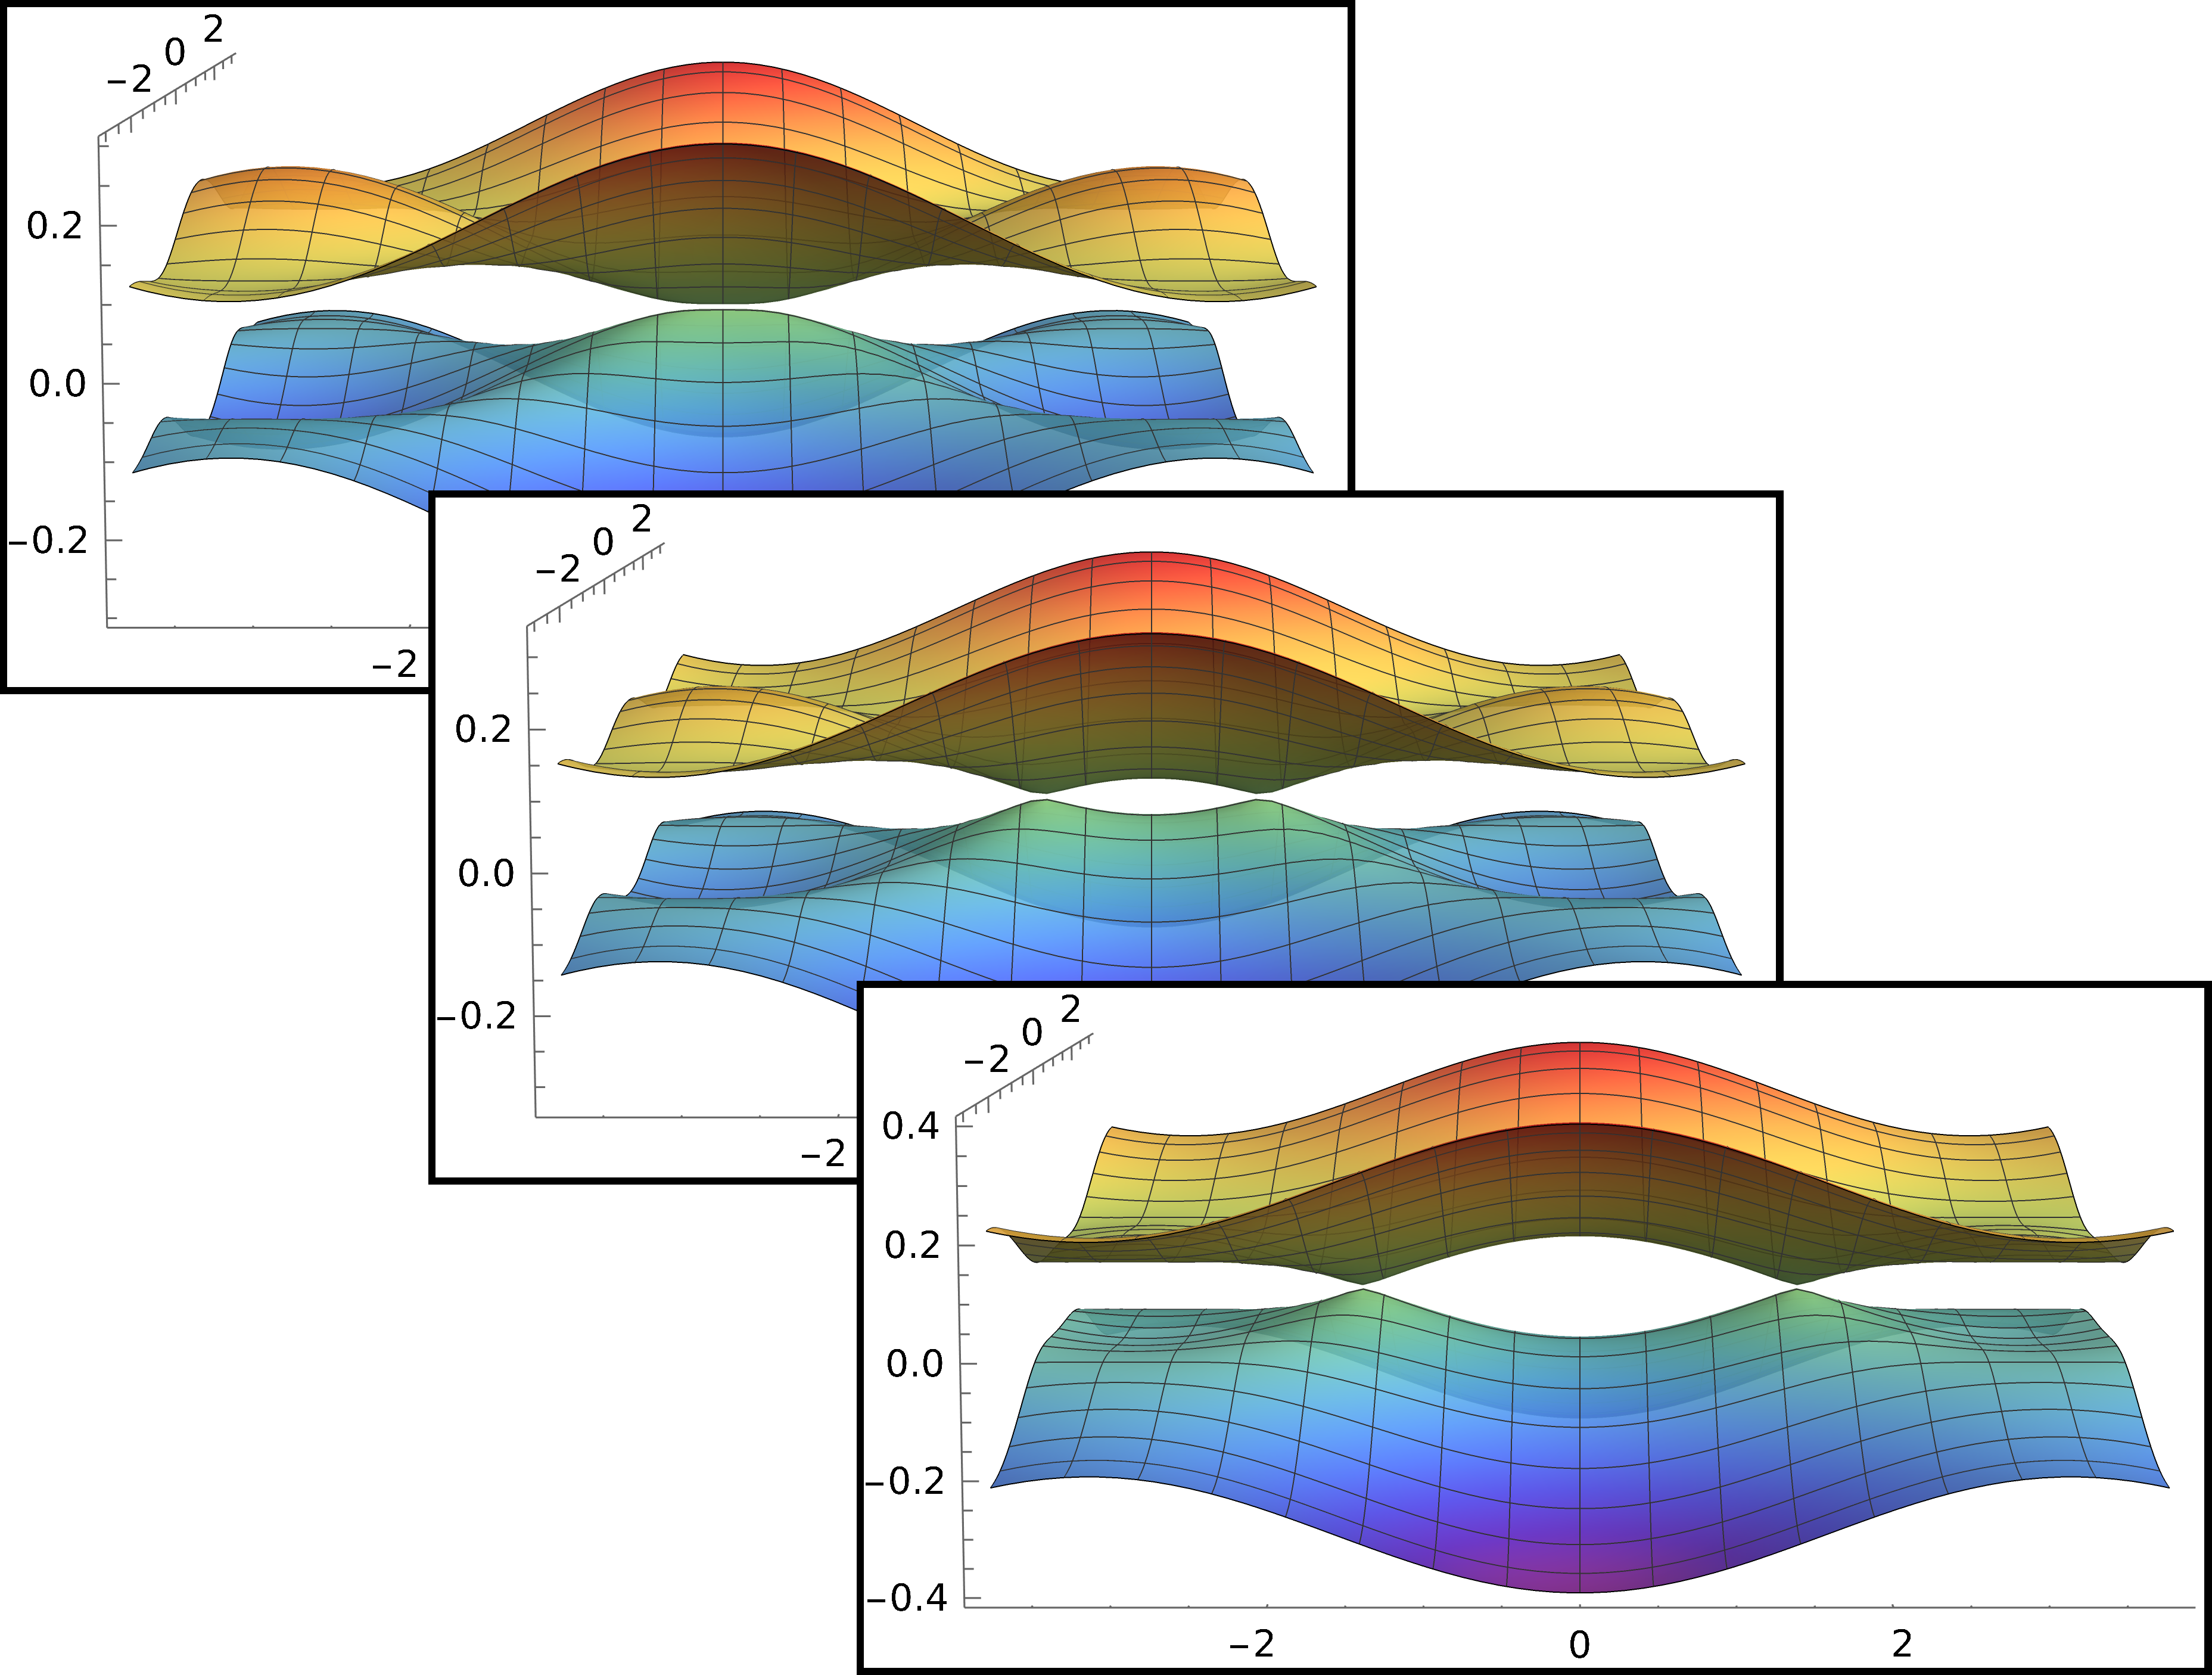
\includegraphics[width=0.7\textwidth]{figures/movetypeiinode}
    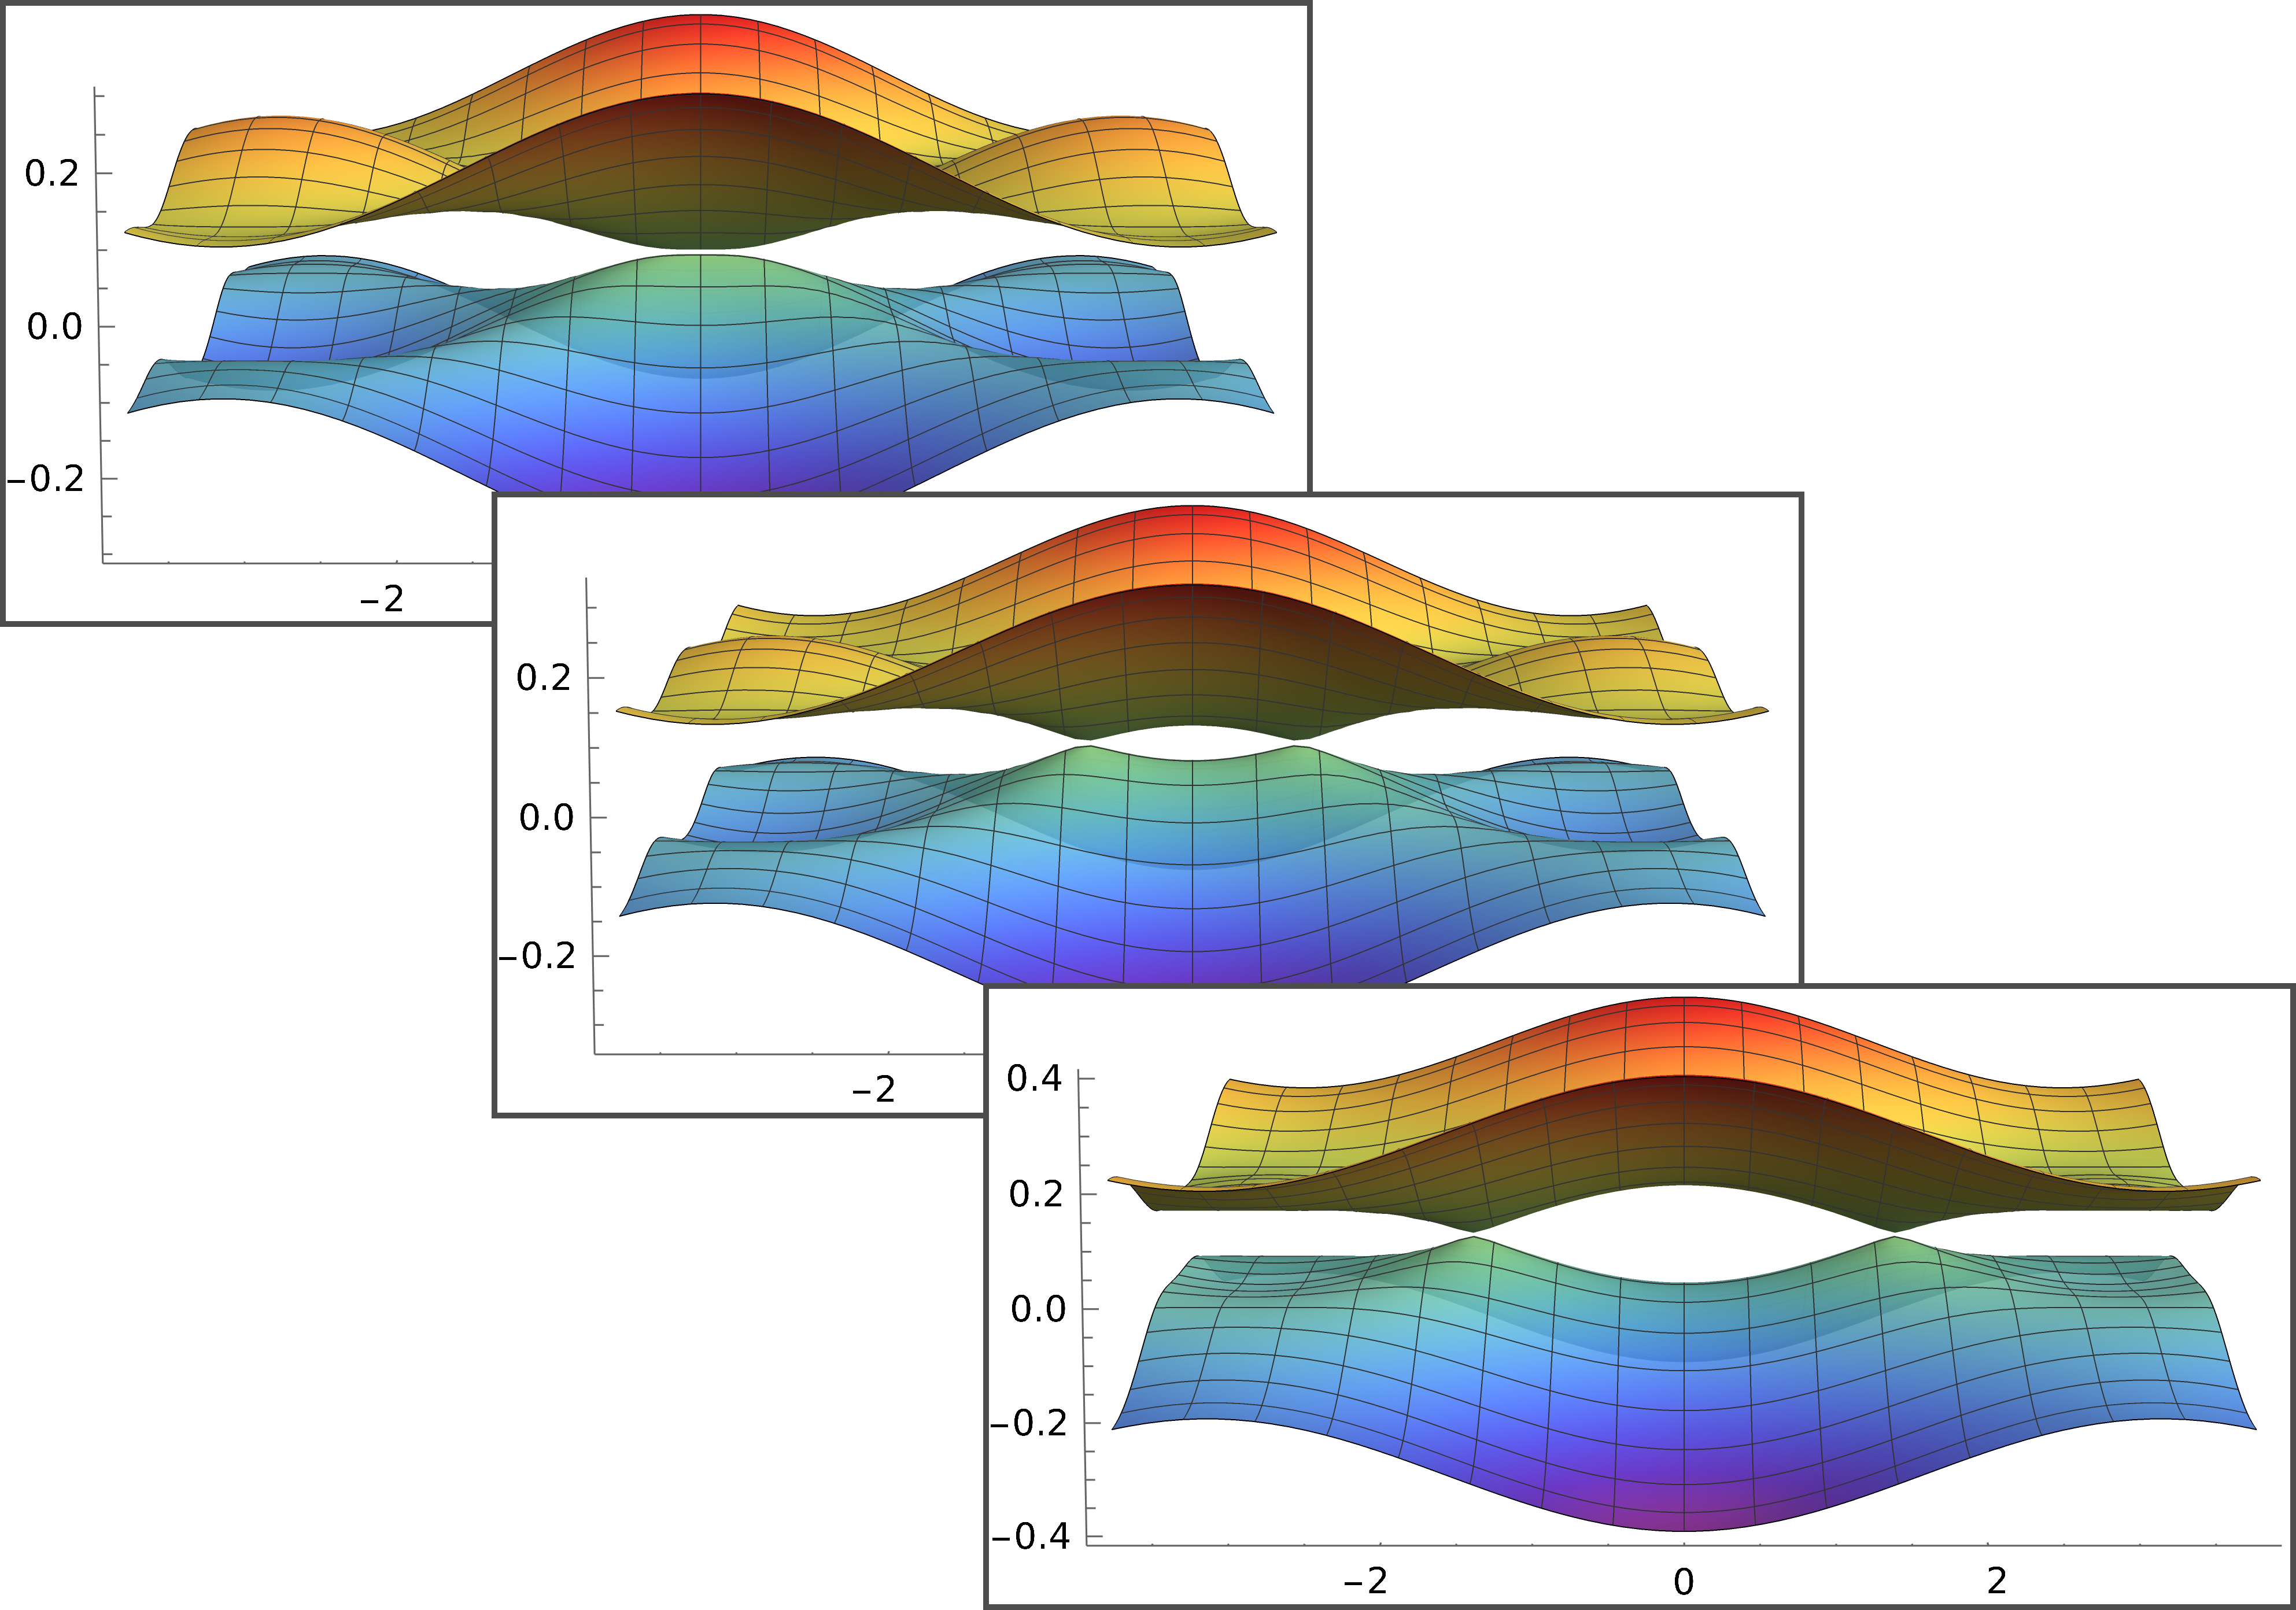
\includegraphics[width=\textwidth]{figures/typeIImoveTransition}
    \caption{\label{fig:typeii:move-nodes} A Type-II Weyl semimetal with separation between the nodes \(2k_{0} = 0, \pi/2, \pi \).
      See main text for details about the model.}
  \end{subcaptionblock}
% \end{figure}
% \begin{figure}[!htb]
  \begin{subcaptionblock}[t]{0.49\textwidth}
    \centering
    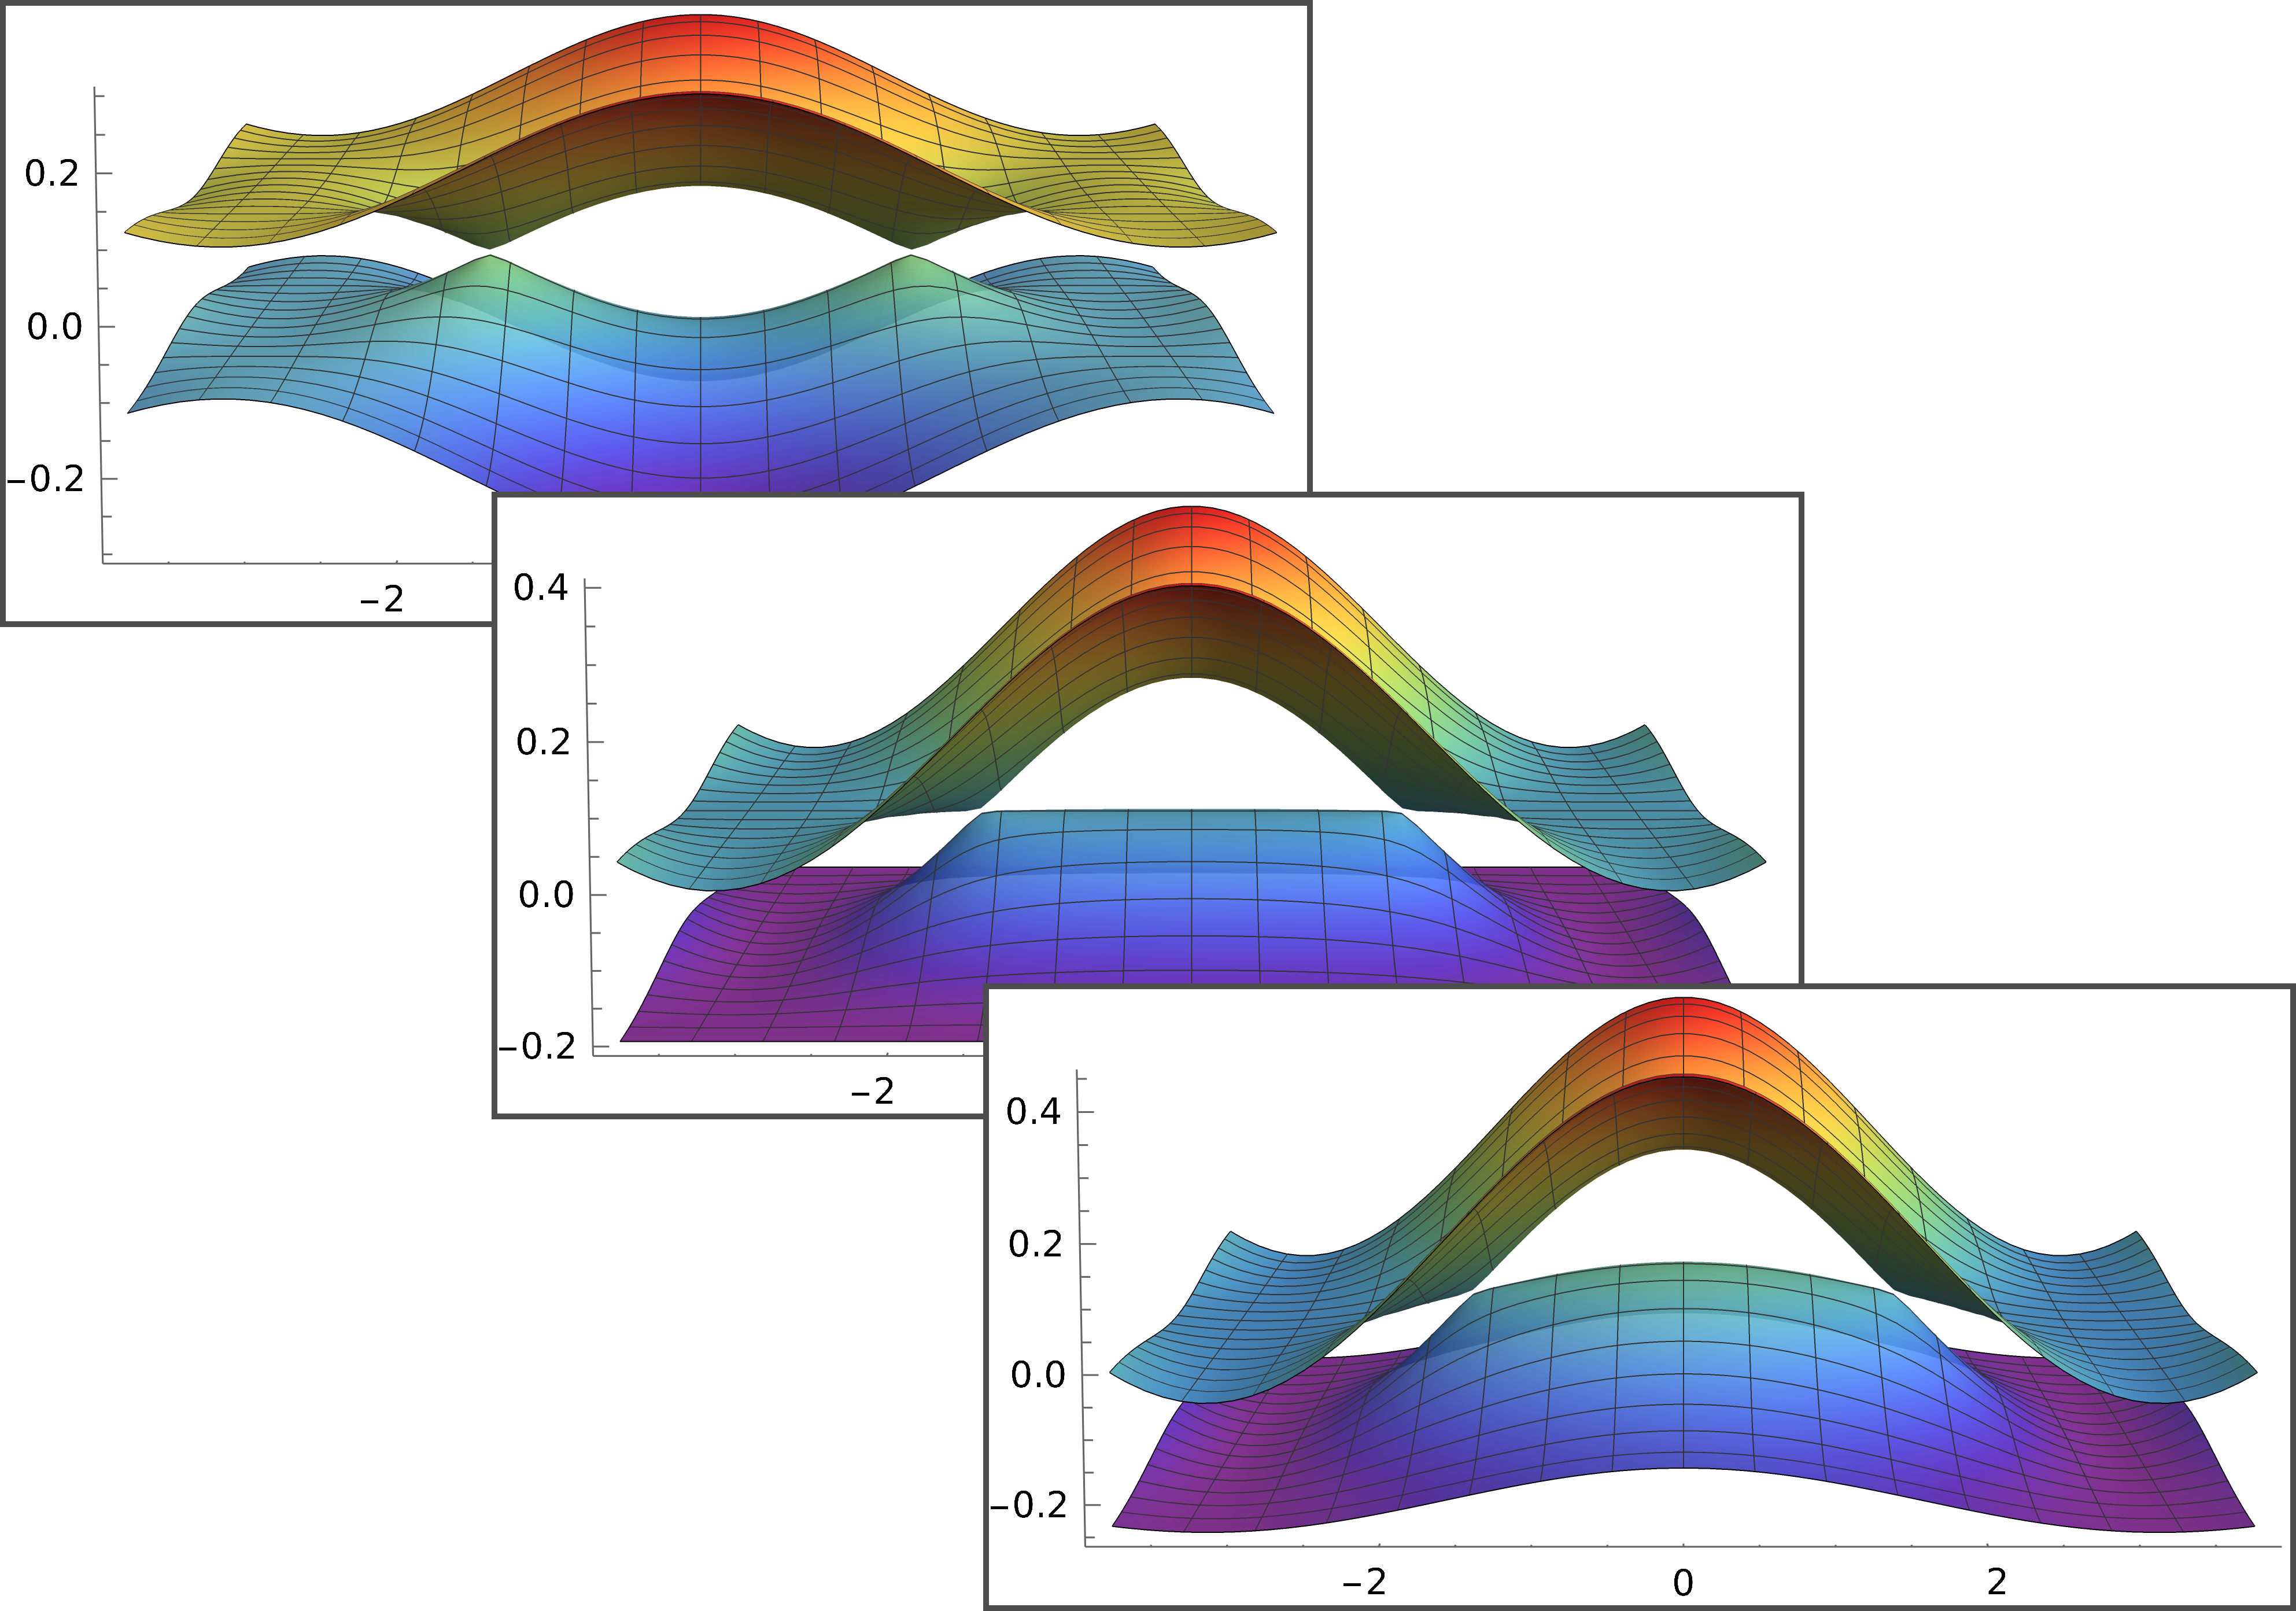
\includegraphics[width=\textwidth]{figures/bendingTransition.png}
    \caption{\label{fig:typeii:bendbands}Tight binding model of tilted Dirac cones, with the parameter \( \gamma \) increased from left to right, transitioning the system from Type-I to Type-II. See main text for details about the model.}
  \end{subcaptionblock}
\end{figure}

Linearizing around the Weyl nodes reduces to the familiar expression of a Dirac cone
\begin{equation}
  \label{eq:7}
  H(\vec{K} ^{'\pm} + \vec{k}) \approx \mp 2 t k_{x} \sin k_{0} \sigma_{1} - 2 t (k_{y} \sigma_{2} + k_{z} \sigma_{3}) \mp \gamma k_{x} \sin k_{0} \sigma_{0}, \: k_{x}, k_{y}, k_{z} \ll 1.
\end{equation}
When the separation between the two nodes is \(\pi\), i.e. \(k_{0} = \pi/ 2 \), the linearized Hamiltonian around the cone is
\begin{equation}
  \label{eq:8}
  H'(\vec{k}) = \mp 2 t k_{x} \sigma_{x} - 2t k_{y} \sigma_{y} - 2 t k_{z} \sigma_{z} \mp \gamma k_{x}.
  % h'(\vec{v}) = -2t \vec{k} \vec{\sigma} - \gamma k_{x}.
\end{equation}
For a system
\begin{equation}
  \label{eq:155}
  H = \gamma_i k_i + k_i A_{ij} \sigma_j,
\end{equation}
the chirality of the node \( s = \det(A_{ij}) \) \cite{mccormickMinimalModelsTopological2017}, and we see this gives a negative cone at \( k_0 = \pi /2 \) and positive at \( k_0 = -\pi /2 \).
We could arrive at a more familiar form of the expression by letting \( 2 t \to v_F, \gamma \to v_F t \), and do a \( \pi \) rotation around \( x \) at the positive cone, giving
\begin{equation}
  \label{eq:158}
  H'(\vec{k}) = s v_F \vec{k} \cdot \vec{\sigma} + s v_F t k_x.
\end{equation}

Moving the two nodes closer together, the effective Fermi velocity in the \(x\)-direction is rescaled, and the system is anisotropic even for no tilt (\(\gamma=0\)).
As discussed earlier, this may be mitigated by a rescaling of \( k_x \).
\todo{make sure this is discussed earlier}
The model thus gives rise to a pair of Weyl cones, with an inversion symmetric tilt, i.e. they tilt with equal magnitude in the opposite direction.

% \begin{figure}[ht]
%   \centering
%   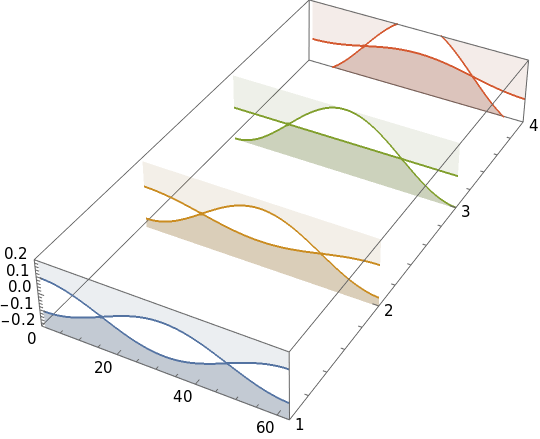
\includegraphics[width=0.7\textwidth]{figures/typeIIridgeline}
%   \caption{The values of the parameters were chosen to be \(m=0.15, t=-0.05, \) and \(2 k_{0}=\pi\).\label{fig:ridgeline}\todo{Write this}}
% \end{figure}

\begin{figure}[ht]
  \centering
  \tikzsetnextfilename{ridgeline}
  \begin{tikzpicture}
    \pgfplotscreateplotcyclelist{myexotic}{
      teal,fill=teal!80!black\\
      orange,fill=orange!80!black\\
      cyan!60!black,fill=cyan!80!black\\
      lime!80!black,fill=lime\\
      red,fill=red!80!black\\
      yellow!60!black,fill=yellow!80!black\\
      black,fill=gray\\
      red,fill=red!80!black\\
    }
    \begin{axis}[
      area plot/.style={
        fill opacity=0.75,
        % draw=#1!80!black,thick,
        % fill=#1,
        mark=none,
      },
      cycle list name={myexotic},
      plot box ratio=3 5 1,
      view={-40}{20},
      zmin=-0.2, zmax=0.2,
      xlabel=\( k_x \),
      ylabel=\( \gamma \),
      zlabel=Energy,
      xtick={-3.1415,-1.5708,0,1.5708,3.1415},
      xticklabels={\( -\pi \), \( -\frac{\pi}{2} \), 0, \( \frac{\pi}{2} \), \( \pi \)},
      ytick={1,2,3,4},
      yticklabels={0,0.05,0.1,0.15},
      ]

      % \addplot3[area plot=orange] table[z index=1, y expr=1, col sep=comma] {data/tightBindModel-topbottom.csv};
      % \addplot3[area plot=orange] table[z index=2, y expr=1, col sep=comma] {data/tightBindModel-topbottom.csv};

      % \addplot3[area plot=blue] table[z index=3, y expr=2, col sep=comma] {data/tightBindModel-topbottom.csv};
      % \addplot3[area plot=blue] table[z index=4, y expr=2, col sep=comma] {data/tightBindModel-topbottom.csv};

      % \addplot3[area plot=teal] table[z index=5, y expr=3, col sep=comma] {data/tightBindModel-topbottom.csv};
      % \addplot3[area plot=teal] table[z index=6, y expr=3, col sep=comma] {data/tightBindModel-topbottom.csv};

      % \addplot3[area plot=teal] table[z index=7, y expr=4, col sep=comma] {data/tightBindModel-topbottom.csv};
      % \addplot3[area plot=teal] table[z index=8, y expr=4, col sep=comma] {data/tightBindModel-topbottom.csv};


      \addplot3+[forget plot, area plot=teal] table[z index=7, y expr=4, col sep=comma] {data/tightBindModel-topbottom.csv};
      \addplot3+[area plot=teal] table[z index=8, y expr=4, col sep=comma] {data/tightBindModel-topbottom.csv};

      \addplot3+[forget plot, area plot=teal] table[z index=5, y expr=3, col sep=comma] {data/tightBindModel-topbottom.csv};
      \addplot3+[area plot=teal] table[z index=6, y expr=3, col sep=comma] {data/tightBindModel-topbottom.csv};

      \addplot3+[forget plot, area plot=blue] table[z index=3, y expr=2, col sep=comma] {data/tightBindModel-topbottom.csv};
      \addplot3+[area plot=blue] table[z index=4, y expr=2, col sep=comma] {data/tightBindModel-topbottom.csv};

      \addplot3+[forget plot, area plot=orange] table[z index=1, y expr=1, col sep=comma] {data/tightBindModel-topbottom.csv};
      \addplot3+[area plot=orange] table[z index=2, y expr=1, col sep=comma] {data/tightBindModel-topbottom.csv};
    \end{axis}
  \end{tikzpicture}
  \caption{The values of the parameters were chosen to be \(m=0.15, t=-0.05, \) and \(2 k_{0}=\pi\).\label{fig:ridgeline2}\todo{Write this}}
\end{figure}


The linearized model are accurate in describing low energy interactions around the Fermi level.
For higher energies their validity falls apart, and more complex models are warranted.
For our calculations, we will take the linear model to be sufficient.
It is much easier to work with, and sufficient in most cases.

% In our calculations the linear models is sufficient, and much easier to work with, and we will thus mainly consider the linear model from here on.
\todo{Fermi surface when tilt, cutoff, finite sea ....}

\subsubsection{The tilt term -- symmetries and Type-I vs.\! Type-II}
For tilted Dirac cones we will consider the Hamiltonian
\begin{equation}
  \label{eq:10}
  H =  s v_F \vec{k} \vec{\sigma} + v_F \vec{t}^s \vec{k},
\end{equation}
where \( s \) denotes the chirality of the Dirac cone, \( v_F \) is the Fermi velocity, and \( \vec{t} \) is the \emph{tilt vector}.
In general the Fermi velocity is anisotropic, as was the case in the general Dirac Hamiltonian given in Eq. \eqref{eq:4}.
By an anisotropic scaling of the momenta \( \vec{k} \), the system may always be mapped to an isotropic case, which we will consider here.

The tilt vector will in general depend on the chirality of the cone.
As the cones always appear in pairs, \( \vec{t}^s = s \vec{t} \) will give a system with inversion symmetry, as was the result from the tight binding model in the subsection on \emph{\nameref{sec:tilt:tightbindingmodel}}.
In the case of broken inversion symmetry, we will consider the case of a tilt equal in direction and magnitude between the two cones, \( \vec{t}^s = \vec{t} \).
In short, we define
\begin{equation}
  \vec{t}^s =
  \begin{cases}
    \vec{t} & \text{broken inversion symmetry},\\
    s \vec{t} & \text{inversion symmetry}.
  \end{cases}\label{eq:11}
\end{equation}
This convention is used in most literature \cite{vanderwurffMagnetovorticalThermoelectricTransport2019,ferreirosAnomalousNernstThermal2017}.

With no magnetic field, the eigenvalues of the system are
\begin{equation}
  \label{eq:12}
  E(\vec{k}) = \vec{\omega_{0}} \vec{k} \pm \sqrt{(v_{i} k_{i})^{2}} = \sqrt{(t_{i} v_{i} k_{i})^{2}} \pm \sqrt{(v_{i} k_{i})^{2}},
\end{equation}
where in the literature the first term is sometimes referred to as the \emph{kinetic} term while the latter is the \emph{potential} term.
The definition for the system to be Type-II is that there exists a direction in momentum space for which the kinetic term dominates over the potential term \cite{soluyanovTypeIIWeylSemimetals2015}.
The \(\vec{t}\)-vector is thus a convenient tool for categorization -- if \(t > 1\) we have a Type-II, else we have a Type-I.


\begin{Proof}
  We may always rotate our coordinate system such that, without loss of generality, \(\vec{t} = t \hat{x}\).
  In that case, the first term obviously dominates in the \(x\)-direction, when $t>1$.
\end{Proof}

\begin{itemize}
  \item In this model, the hole pocket is ``shared'' between the two cones. There are also models with individual pockets (see \cite{mccormickMinimalModelsTopological2017})
\end{itemize}


